\documentclass[12pt]{article}

% ── Page geometry ────────────────────────────────────────────────────────────
\usepackage[a4paper, margin=1in]{geometry}
\usepackage{setspace}
\singlespacing

% ── Fonts & encoding ────────────────────────────────────────────────────────
\usepackage[T1]{fontenc}
\usepackage[utf8]{inputenc}
\usepackage{lmodern}

% ── Packages ─────────────────────────────────────────────────────────────────
\usepackage{graphicx}
\usepackage{booktabs}
\usepackage{multirow}
\usepackage{amsmath, amssymb}
\usepackage{hyperref}
\usepackage{xcolor}
\usepackage{enumitem}
\usepackage{caption}
\usepackage{subcaption}
\usepackage{float}
\usepackage{listings}
\usepackage{xurl}

\hypersetup{
    colorlinks=true,
    linkcolor=blue!70!black,
    citecolor=blue!70!black,
    urlcolor=blue!70!black,
}

\captionsetup{font={small}, labelfont={bf}}

% ── Code listing style ──────────────────────────────────────────────────────
\lstset{
    language=Python,
    basicstyle=\ttfamily\scriptsize,
    keywordstyle=\color{blue!70!black}\bfseries,
    commentstyle=\color{green!50!black}\itshape,
    stringstyle=\color{red!60!black},
    numbers=left,
    numberstyle=\tiny\color{gray},
    numbersep=5pt,
    frame=single,
    framesep=3pt,
    breaklines=true,
    breakatwhitespace=false,
    showstringspaces=false,
    tabsize=4,
    captionpos=b,
    xleftmargin=1.5em,
    framexleftmargin=1.5em,
}

% ── Title ────────────────────────────────────────────────────────────────────
\title{%
    \textbf{Corporate Evasion Decoder:}\\[4pt]
    \large Detecting Evasive Communication in\\
    Earnings Call Q\&A Sessions
}
\author{
    NYCU --- Artificial Intelligence, Spring 2026\\[2pt]
    Homework 1: Dataset Construction \& Analysis
}
\date{}

% ═════════════════════════════════════════════════════════════════════════════
\begin{document}
\maketitle
\thispagestyle{empty}

\noindent\textbf{GitHub:}
\url{https://github.com/YOUR-USERNAME/CorporateEvasionDecoder}

% ─────────────────────────────────────────────────────────────────────────────
\section{Research Question and Motivation}
% ─────────────────────────────────────────────────────────────────────────────

Corporate earnings calls are a primary channel through which public companies
communicate financial performance to investors and analysts. During the Q\&A
portion, executives may respond with varying degrees of transparency: some
answers are direct and data-driven, while others employ hedging language,
excessive jargon, or strategic vagueness to deflect difficult questions.
Detecting such evasive communication is valuable for financial analysts,
regulators, and NLP researchers.

We pose the following research question: \emph{Can we automatically classify
corporate Q\&A responses as \textsc{Direct}, \textsc{Evasive}, or
\textsc{Jargon}-heavy using a combination of handcrafted linguistic features
and text representations?}

This task is challenging for several reasons. First, evasiveness is inherently
subjective---reasonable annotators may disagree. Second, corporate language is
domain-specific, and jargon that signals evasiveness in one context may be
perfectly appropriate in another. Third, the dataset is modest in size
(\(n = 1{,}129\)), making high-capacity models prone to overfitting. These
challenges make the project an ideal testbed for comparing classical ML
approaches against a fine-tuned transformer under realistic data constraints.

% ─────────────────────────────────────────────────────────────────────────────
\section{Dataset Documentation}
% ─────────────────────────────────────────────────────────────────────────────

\subsection{Data Type and Source}

Each sample is a \textbf{question--answer pair} extracted from public earnings
call transcripts. The text is in English and drawn from formal corporate
communication. Transcripts were obtained from \textbf{SeekingAlpha}
via the RapidAPI endpoint
\texttt{seeking-alpha.p.rapidapi.com}~\cite{seekingalpha}.

\subsection{Amount and Composition}

\begin{table}[H]
\centering
\caption{Dataset composition by label.}
\label{tab:class_dist}
\begin{tabular}{lrr}
\toprule
\textbf{Label} & \textbf{Count} & \textbf{Proportion} \\
\midrule
\textsc{Direct}  & 395 & 35.0\% \\
\textsc{Evasive} & 352 & 31.2\% \\
\textsc{Jargon}  & 382 & 33.8\% \\
\midrule
\textbf{Total}   & 1{,}129 & 100.0\% \\
\bottomrule
\end{tabular}
\end{table}

The dataset spans \textbf{20 companies} across \textbf{6 sectors}:
Technology (AAPL, MSFT, GOOGL, META, AMZN, NVDA),
Finance (JPM, GS, BAC),
Healthcare (JNJ, PFE, UNH),
Consumer (PG, KO, WMT, MCD),
Energy (XOM, CVX),
and Industrial (CAT, GE).
A total of 131 transcripts were crawled, of which 87 contained extractable
Q\&A sections, yielding 1{,}129 pairs. Table~\ref{tab:class_dist} shows the
well-balanced class distribution, with each label comprising roughly one-third
of the data.

\begin{figure}[H]
    \centering
    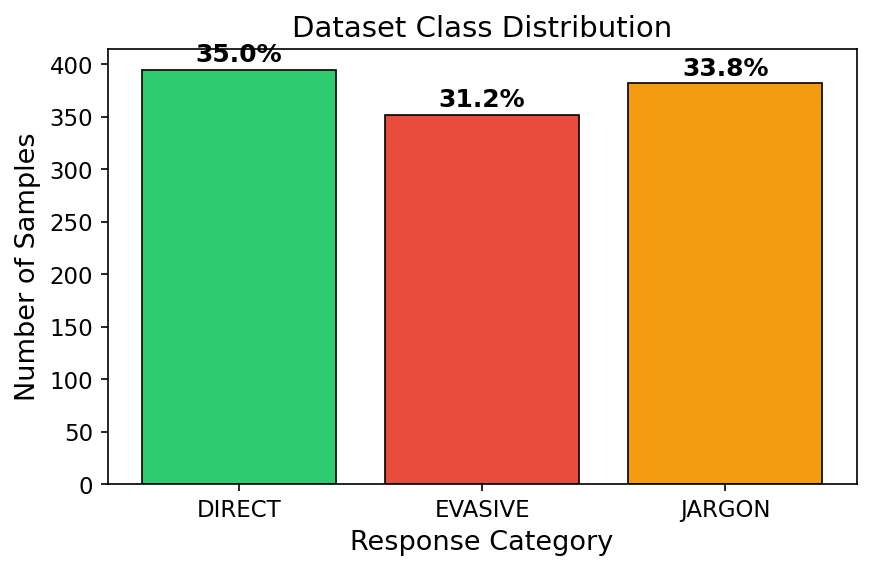
\includegraphics[width=0.55\textwidth]{../figures/fig_class_distribution.png}
    \caption{Class distribution across the three labels.}
    \label{fig:class_dist}
\end{figure}

\subsection{Collection Process}

Data collection followed a four-stage pipeline:
\begin{enumerate}[nosep]
    \item \textbf{Crawling.} For each of the 20 tickers, up to 8 recent
          earnings call transcript IDs were retrieved via the SeekingAlpha API.
          Full HTML transcripts were then downloaded (131 total, capped at
          480 API calls).
    \item \textbf{Q\&A extraction.} HTML transcripts were parsed to isolate
          the Q\&A section. Speaker turns were segmented by
          \texttt{<p>} tags with speaker-name formatting. Analyst questions
          were paired with the subsequent executive answer, yielding
          structured \texttt{(question, answer, ticker, date)} tuples.
    \item \textbf{LLM annotation.} Each Q\&A pair was classified by
          \textbf{Qwen3-8B}~\cite{qwen} running locally with zero-shot
          prompting. The prompt asked the model to assign exactly one of
          three labels---\textsc{Direct}, \textsc{Evasive}, or
          \textsc{Jargon}---based on explicit criteria (e.g., hedging
          language, numerical specificity, buzzword density). This
          semi-automatic approach enabled labeling the full dataset
          consistently while acknowledging that label noise is inevitable.
    \item \textbf{Feature engineering.} Two feature families were computed:
          500-dimensional TF-IDF vectors (unigrams + bigrams) and 21
          handcrafted linguistic features (see Section~\ref{sec:features}).
\end{enumerate}

\subsection{Conditions and Limitations}

Transcripts are public, sourced from a commercial API, and contain no
personally identifiable information beyond public executive names. The
LLM-generated labels introduce systematic noise: the annotator has no
ground-truth human labels for calibration. We acknowledge this as the
primary limitation and discuss its impact on model performance in
Section~\ref{sec:discussion}.

\subsection{Examples}

\begin{itemize}[nosep]
    \item \textbf{Direct:} \emph{``Revenue grew 12\% year-over-year to
          \$23.4 billion, driven primarily by cloud services which grew
          28\%.''}
    \item \textbf{Evasive:} \emph{``We continue to evaluate our strategic
          options and remain focused on long-term value creation for our
          stakeholders across the portfolio.''}
    \item \textbf{Jargon:} \emph{``We're leveraging our synergistic
          ecosystem to drive paradigm-shifting innovation across
          verticals.''}
\end{itemize}

% ─────────────────────────────────────────────────────────────────────────────
\section{Feature Engineering}
\label{sec:features}
% ─────────────────────────────────────────────────────────────────────────────

The feature space comprises \textbf{521 dimensions}: 500 TF-IDF features and
21 handcrafted linguistic features designed to capture communication style
beyond bag-of-words statistics.

\begin{table}[H]
\centering
\caption{The 21 handcrafted linguistic features grouped by category.}
\label{tab:features}
\small
\begin{tabular}{llp{6.5cm}}
\toprule
\textbf{Category} & \textbf{Feature} & \textbf{Description} \\
\midrule
\multirow{5}{*}{Length}
    & \texttt{answer\_word\_count}      & Word count of the answer \\
    & \texttt{answer\_sent\_count}      & Sentence count of the answer \\
    & \texttt{avg\_sent\_length}        & Average sentence length (words) \\
    & \texttt{question\_word\_count}    & Word count of the question \\
    & \texttt{qa\_length\_ratio}        & Answer length / question length \\
\midrule
\multirow{2}{*}{Hedging}
    & \texttt{hedge\_word\_count}       & Count of hedge words (\emph{might, could, possibly, generally}, etc.) \\
    & \texttt{hedge\_word\_ratio}       & Proportion of hedge words \\
\midrule
\multirow{2}{*}{Jargon}
    & \texttt{jargon\_word\_count}      & Count of corporate jargon (\emph{synergy, leverage, ecosystem}, etc.) \\
    & \texttt{jargon\_word\_ratio}      & Proportion of jargon words \\
\midrule
\multirow{4}{*}{Specificity}
    & \texttt{number\_count}            & Count of numeric tokens \\
    & \texttt{number\_ratio}            & Proportion of numeric tokens \\
    & \texttt{metric\_count}            & Count of metric phrases (e.g., \emph{\$X billion}) \\
    & \texttt{metric\_ratio}            & Proportion of metric phrases \\
\midrule
\multirow{2}{*}{Pronouns}
    & \texttt{first\_person\_ratio}     & Ratio of first-person pronouns \\
    & \texttt{third\_person\_ratio}     & Ratio of third-person pronouns \\
\midrule
\multirow{2}{*}{Complexity}
    & \texttt{avg\_word\_length}        & Average word length (characters) \\
    & \texttt{long\_word\_ratio}        & Proportion of words $\geq 7$ characters \\
\midrule
\multirow{2}{*}{Structure}
    & \texttt{starts\_with\_direct\_answer} & Binary: starts with yes/no/number \\
    & \texttt{question\_keyword\_overlap}   & Jaccard overlap of Q\&A keywords \\
\midrule
Semantic
    & \texttt{qa\_tfidf\_similarity}    & Cosine similarity between Q\&A TF-IDF vectors \\
\bottomrule
\end{tabular}
\end{table}

The TF-IDF features were extracted from the concatenated question--answer
text using scikit-learn's \texttt{TfidfVectorizer}~\cite{sklearn} with a
maximum of 500 features (unigrams and bigrams). The handcrafted features
capture stylistic and structural properties that are hypothesized to
discriminate between direct, evasive, and jargon-heavy responses.

% ─────────────────────────────────────────────────────────────────────────────
\section{Methods}
\label{sec:methods}
% ─────────────────────────────────────────────────────────────────────────────

We evaluate four classifiers spanning a spectrum from linear models to
deep pre-trained transformers. The goal is to compare (i)~\textbf{feature-based
classical ML}---which can work well in low-data regimes and is easy to
interpret---against (ii)~a \textbf{pre-trained transformer} that learns
representations directly from raw text. All classical models use the full
521-feature representation; DistilBERT operates on raw text.

\paragraph{Deep-learning constraint.}
Per the assignment requirement (\emph{at most one model can be deep-learning based}),
we include exactly \textbf{one} neural model (DistilBERT) and compare it against
\textbf{three} classical supervised baselines (LR, SVM, XGBoost).

\paragraph{Logistic Regression (LR).}
Multinomial logistic regression with L2 regularization, solved via L-BFGS.
LR serves as a transparent linear baseline: if evasion cues are largely
additive (e.g., more hedging words, fewer numbers), a linear separator can
perform competitively while remaining easy to inspect via feature weights.

\paragraph{Support Vector Machine (SVM).}
SVM with an RBF kernel ($C = 1.0$, $\gamma = \text{scale}$), using
one-vs-rest decomposition with Platt scaling for probability estimates.
The RBF kernel maps features to an implicit high-dimensional space,
capturing nonlinear decision boundaries.

\paragraph{XGBoost.}
Gradient-boosted decision trees~\cite{xgboost} with 100 estimators,
maximum depth 4, and learning rate 0.1. XGBoost provides built-in
feature importance via gain, enabling interpretability, and is robust to
noisy or irrelevant features through its sequential boosting procedure.

\paragraph{DistilBERT.}
A fine-tuned \texttt{distilbert-base-uncased}~\cite{distilbert} transformer
with a linear classification head. Training used class-weighted
cross-entropy loss (to account for mild imbalance), a learning rate of
$5 \times 10^{-5}$, dropout 0.3, and early stopping (patience 3).
DistilBERT operates on raw text and learns contextual
representations end-to-end, bypassing the need for manual feature
engineering.

\paragraph{Evaluation Protocol.}
All models were evaluated using \textbf{stratified 5-fold cross-validation}
to ensure each fold preserves the class distribution. We report
accuracy, macro-averaged F1 score, and one-vs-rest AUROC (where applicable).
Per-class precision, recall, and F1 are reported for detailed analysis.

% ─────────────────────────────────────────────────────────────────────────────
\section{Experiments and Results}
\label{sec:experiments}
% ─────────────────────────────────────────────────────────────────────────────

\subsection{Experiment 1: Baseline Comparison}

Table~\ref{tab:baseline} presents the baseline performance of all four
models on the full 521-feature set (or raw text for DistilBERT).

\begin{table}[H]
\centering
\caption{Baseline 5-fold cross-validation results (mean $\pm$ std). AUROC is
macro-averaged one-vs-rest.}
\label{tab:baseline}
\small
\begin{tabular}{lccc}
\toprule
\textbf{Model} & \textbf{Accuracy} & \textbf{F1 (macro)} & \textbf{AUROC} \\
\midrule
Logistic Regression & $0.455 \pm 0.027$ & $0.453 \pm 0.026$ & 0.646 \\
SVM (RBF)           & $0.532 \pm 0.037$ & $0.528 \pm 0.036$ & 0.731 \\
XGBoost             & $0.544 \pm 0.029$ & $0.542 \pm 0.030$ & 0.728 \\
DistilBERT          & $\mathbf{0.576 \pm 0.026}$ & $\mathbf{0.570 \pm 0.022}$ & $\mathbf{0.747 \pm 0.038}$ \\
\bottomrule
\end{tabular}
\end{table}

DistilBERT achieves the highest performance, demonstrating that
pre-trained contextual representations provide an advantage over
handcrafted features for this task. Among classical models, XGBoost leads
marginally over SVM, while Logistic Regression lags substantially.

Table~\ref{tab:perclass} breaks down per-class performance for XGBoost.
\textsc{Direct} responses are easiest to detect (F1 = 0.586), likely because
they contain distinctive numerical and factual content.
\textsc{Evasive} and \textsc{Jargon} are harder to distinguish from each
other (F1 $\approx$ 0.52), suggesting overlap in their linguistic signatures.

\begin{table}[H]
\centering
\caption{Per-class metrics for XGBoost (baseline).}
\label{tab:perclass}
\small
\begin{tabular}{lccc}
\toprule
\textbf{Class} & \textbf{Precision} & \textbf{Recall} & \textbf{F1} \\
\midrule
\textsc{Direct}  & 0.571 & 0.603 & 0.586 \\
\textsc{Evasive} & 0.541 & 0.509 & 0.524 \\
\textsc{Jargon}  & 0.517 & 0.516 & 0.516 \\
\bottomrule
\end{tabular}
\end{table}

\begin{figure}[H]
    \centering
    \begin{minipage}[t]{0.48\textwidth}
        \centering
        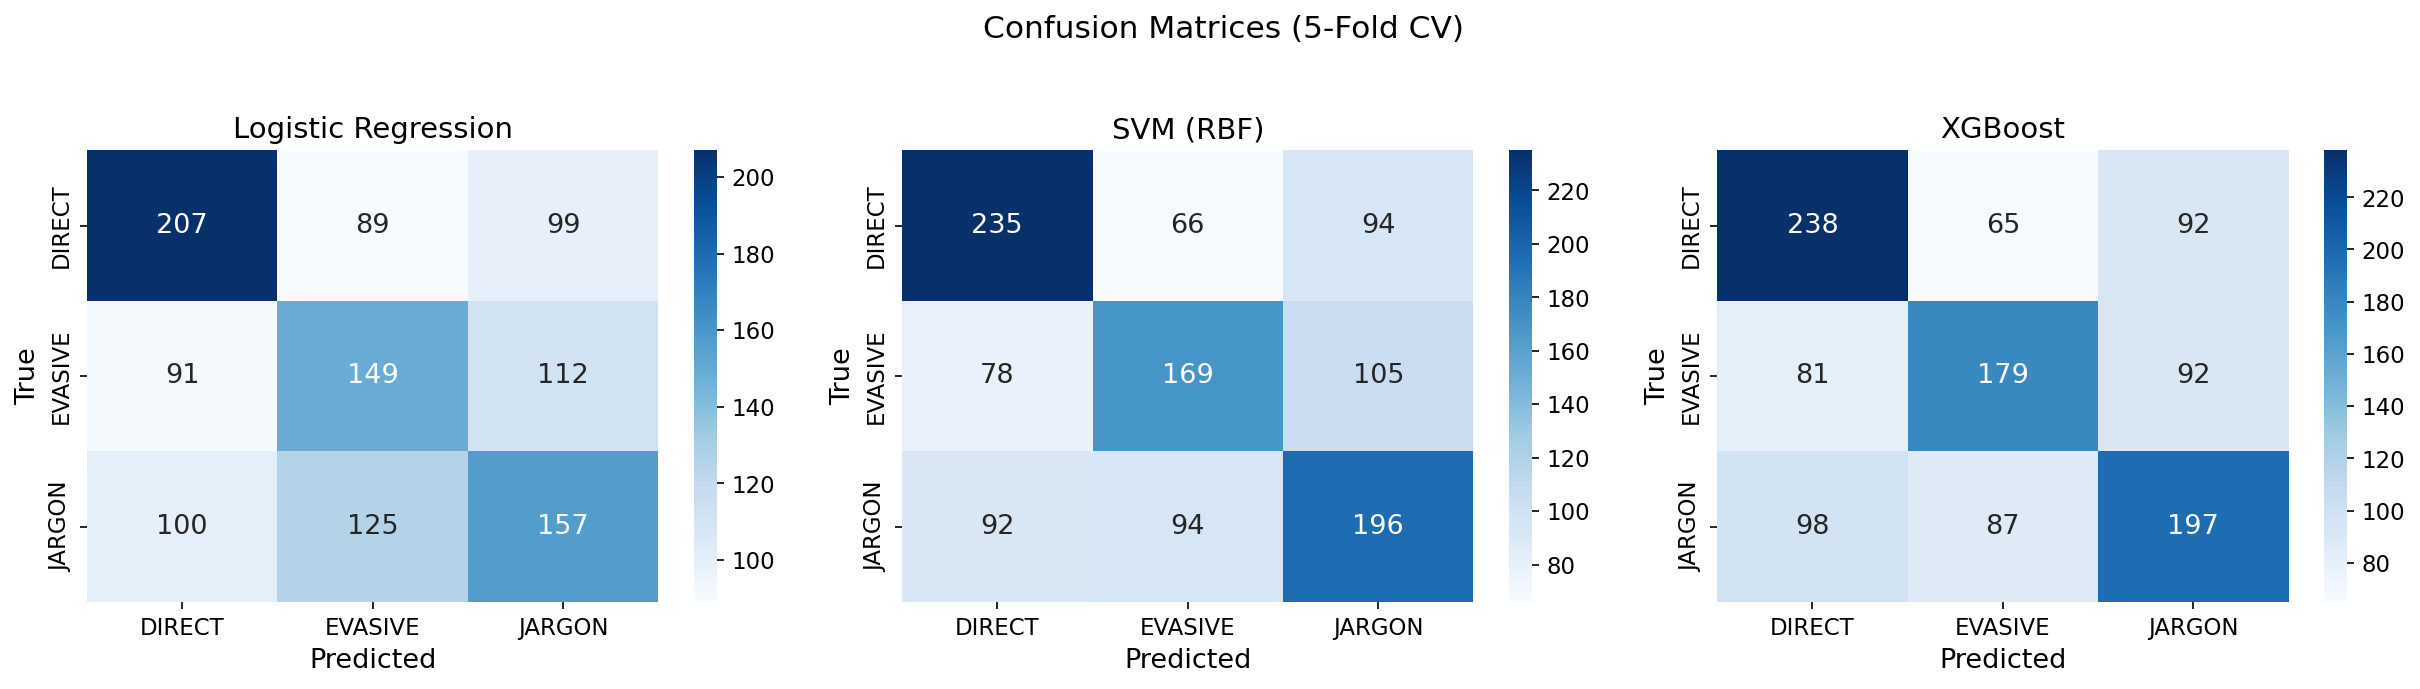
\includegraphics[width=\textwidth]{../figures/fig_confusion_matrices.png}
        \caption{Confusion matrices for classical models.}
        \label{fig:confusion}
    \end{minipage}
    \hfill
    \begin{minipage}[t]{0.48\textwidth}
        \centering
        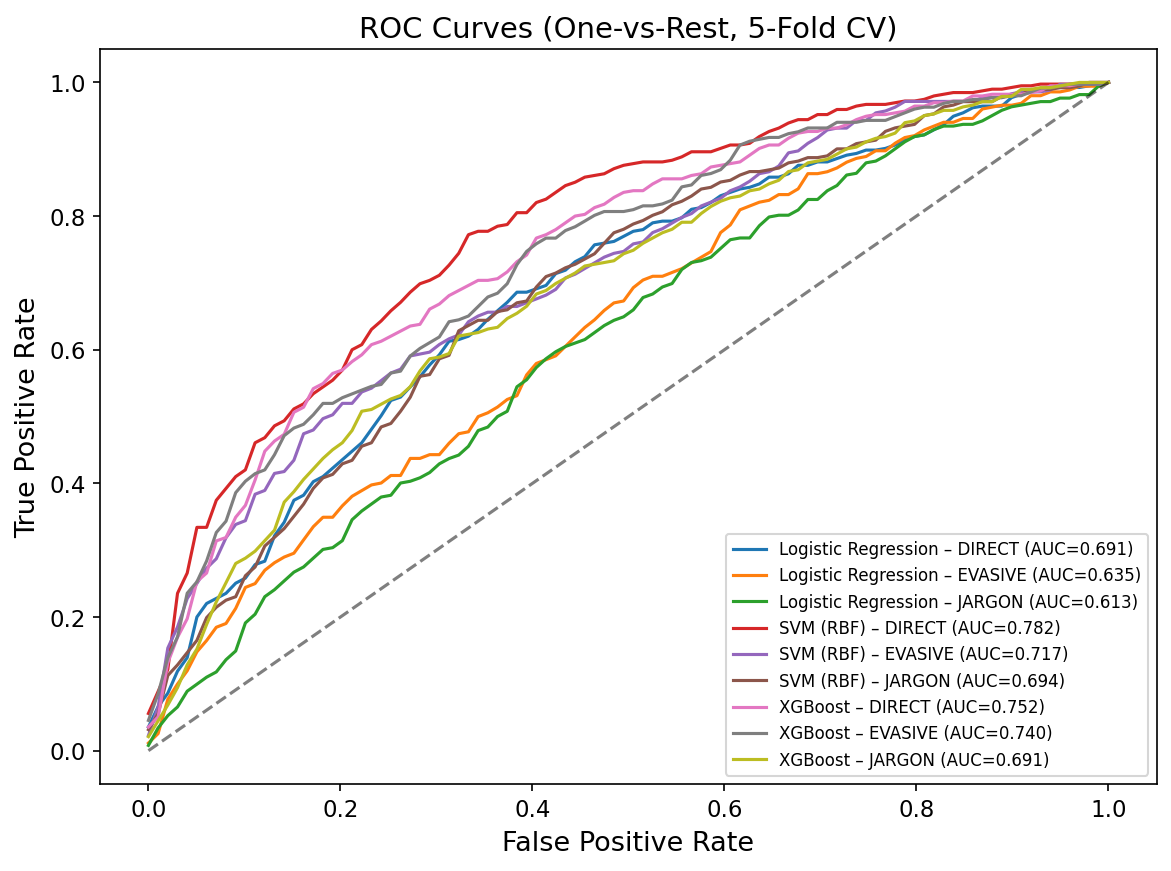
\includegraphics[width=\textwidth]{../figures/fig_roc_curves.png}
        \caption{One-vs-rest ROC curves.}
        \label{fig:roc}
    \end{minipage}
\end{figure}

The confusion matrices (Figure~\ref{fig:confusion}) reveal that
\textsc{Evasive} and \textsc{Jargon} are frequently confused with each
other, consistent with our intuition that both involve non-specific,
non-committal language. The ROC curves (Figure~\ref{fig:roc}) show that
all models achieve AUROC well above 0.5 for each class, confirming that
the features carry discriminative signal despite the modest overall accuracy.

% ── Experiment 2 ─────────────────────────────────────────────────────────────
\subsection{Experiment 2: Learning Curves}

\begin{figure}[H]
    \centering
    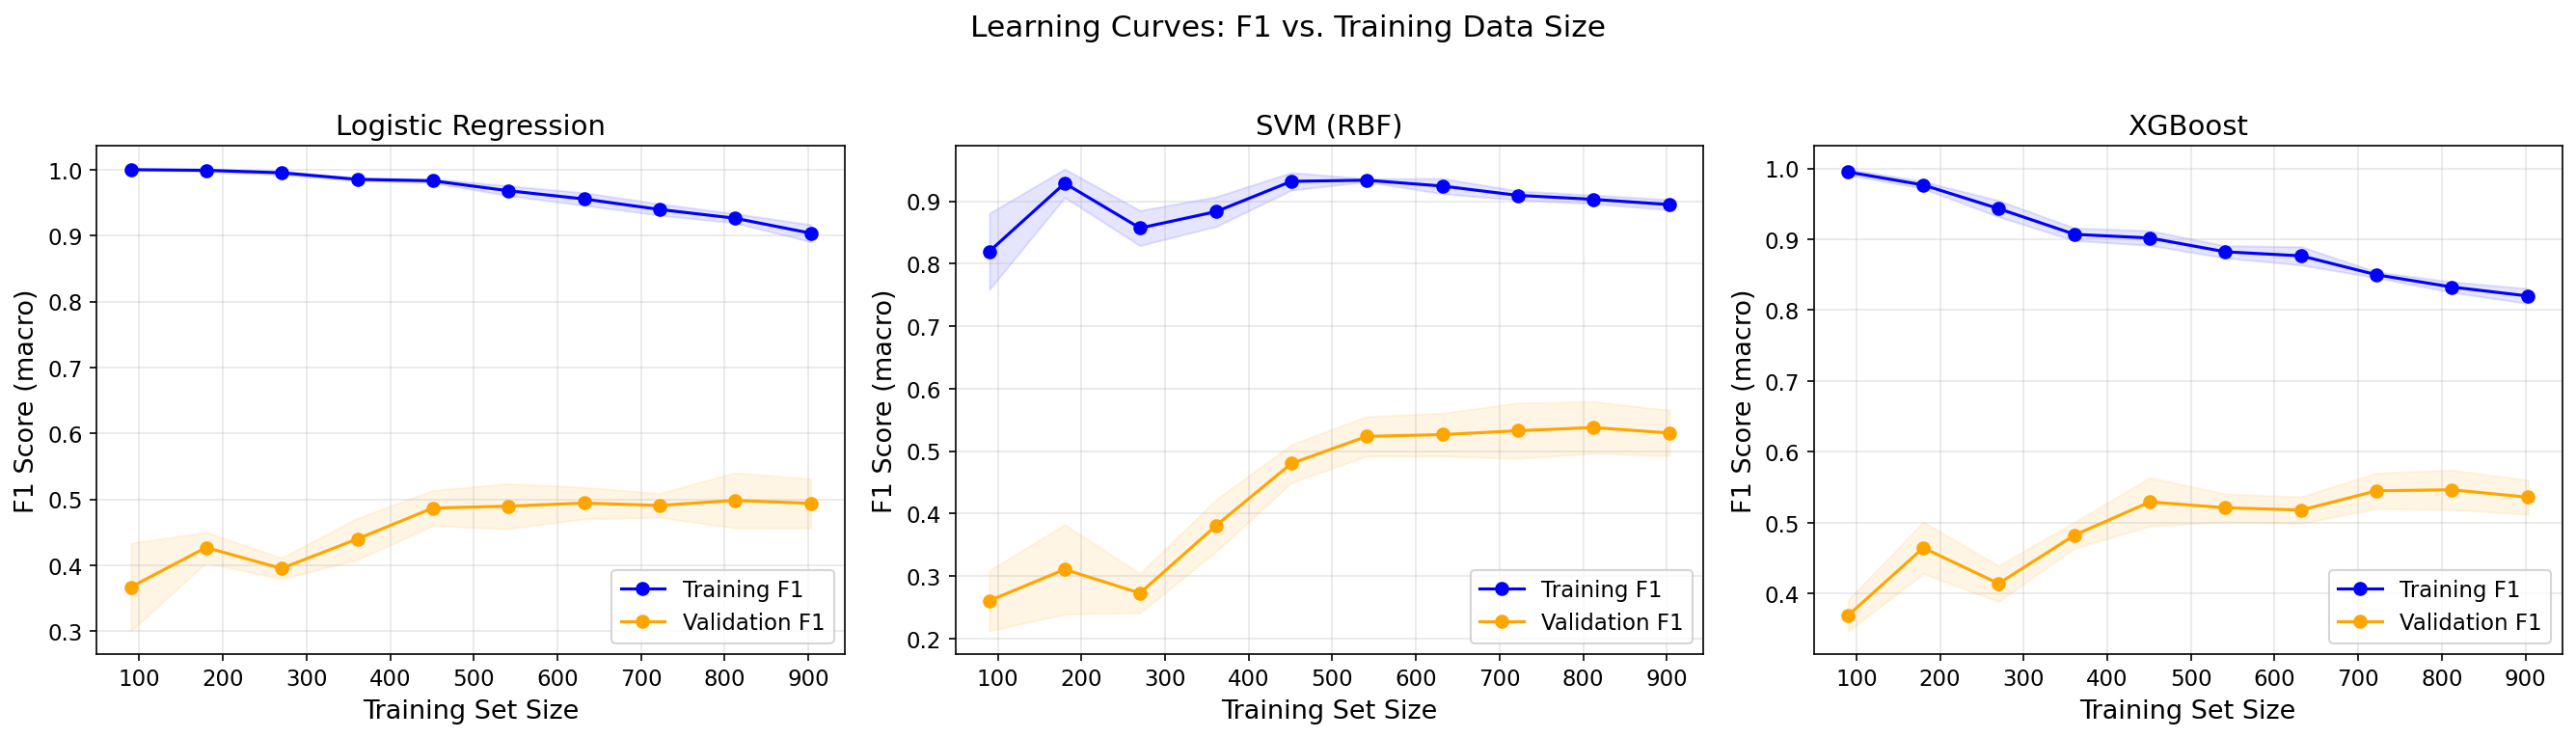
\includegraphics[width=0.85\textwidth]{../figures/fig_learning_curves.png}
    \caption{Learning curves showing training vs.\ validation F1 as a
             function of training set fraction.}
    \label{fig:learning}
\end{figure}

Figure~\ref{fig:learning} shows that all models exhibit a persistent
training--validation gap, indicating overfitting. Validation F1 improves
as more data is added but plateaus around 0.55, suggesting that
performance is bounded not only by model capacity but also by label noise
from the LLM annotator. The upward trend at larger training fractions
indicates that \emph{more data would likely help}, making data augmentation
a natural next step (see Section~\ref{sec:augment}).

% ── Experiment 3 ─────────────────────────────────────────────────────────────
\subsection{Experiment 3: SMOTE Analysis}

Since class imbalance can degrade minority-class performance, we evaluated
SMOTE~\cite{smote} (Synthetic Minority Oversampling Technique) applied
within each cross-validation fold.

\begin{table}[H]
\centering
\caption{Effect of SMOTE on macro-F1.}
\label{tab:smote}
\small
\begin{tabular}{lccc}
\toprule
\textbf{Model} & \textbf{No SMOTE} & \textbf{With SMOTE} & \textbf{$\Delta$} \\
\midrule
Logistic Regression & 0.453 & 0.453 & $-0.000$ \\
SVM (RBF)           & 0.528 & 0.523 & $-0.005$ \\
XGBoost             & 0.542 & 0.546 & $+0.004$ \\
\bottomrule
\end{tabular}
\end{table}

\begin{figure}[H]
    \centering
    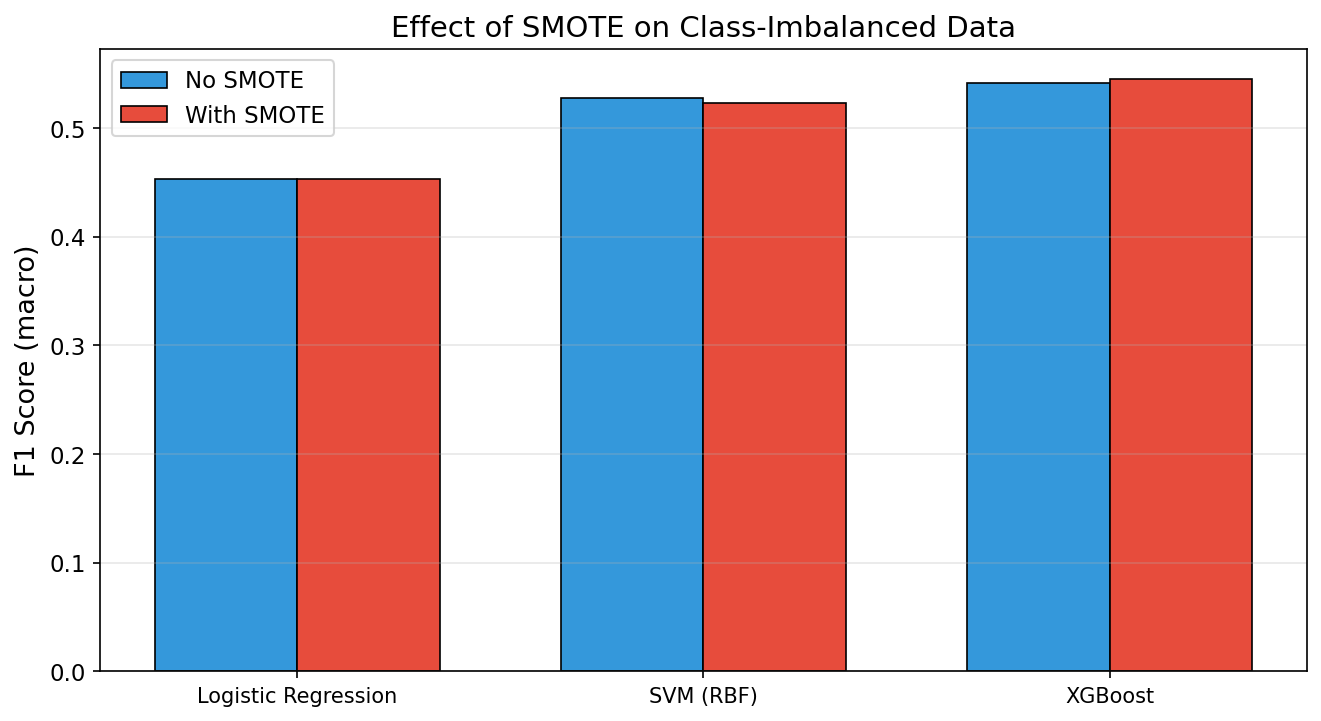
\includegraphics[width=0.55\textwidth]{../figures/fig_smote_comparison.png}
    \caption{SMOTE vs.\ no-SMOTE comparison across models.}
    \label{fig:smote}
\end{figure}

SMOTE produces negligible changes ($|\Delta| < 0.006$) for all models.
This is expected: the dataset is already well-balanced (35/31/34\%), so
oversampling the slightly smaller \textsc{Evasive} class adds little
value. For SVM, the synthetic samples even introduce a slight performance
drop, possibly because SMOTE-generated points near the decision boundary
add noise in high-dimensional feature space. This experiment confirms
that class imbalance is \emph{not} a contributing factor to the moderate
accuracy.

% ── Experiment 4 ─────────────────────────────────────────────────────────────
\subsection{Experiment 4: PCA Dimensionality Reduction}

With 521 features and only 1{,}129 samples, the curse of dimensionality
may harm linear models. We applied PCA to the feature matrix and evaluated
performance at various component counts.

\begin{table}[H]
\centering
\caption{Macro-F1 as a function of PCA components.}
\label{tab:pca}
\small
\begin{tabular}{lccc}
\toprule
\textbf{Components} & \textbf{LR} & \textbf{SVM} & \textbf{XGBoost} \\
\midrule
25              & 0.538          & 0.528          & 0.513          \\
50              & \textbf{0.545} & \textbf{0.534} & 0.529          \\
100             & 0.519          & 0.527          & 0.516          \\
200             & 0.497          & 0.524          & 0.509          \\
521 (full)      & 0.453          & 0.528          & \textbf{0.542} \\
\bottomrule
\end{tabular}
\end{table}

\begin{figure}[H]
    \centering
    \begin{minipage}[t]{0.48\textwidth}
        \centering
        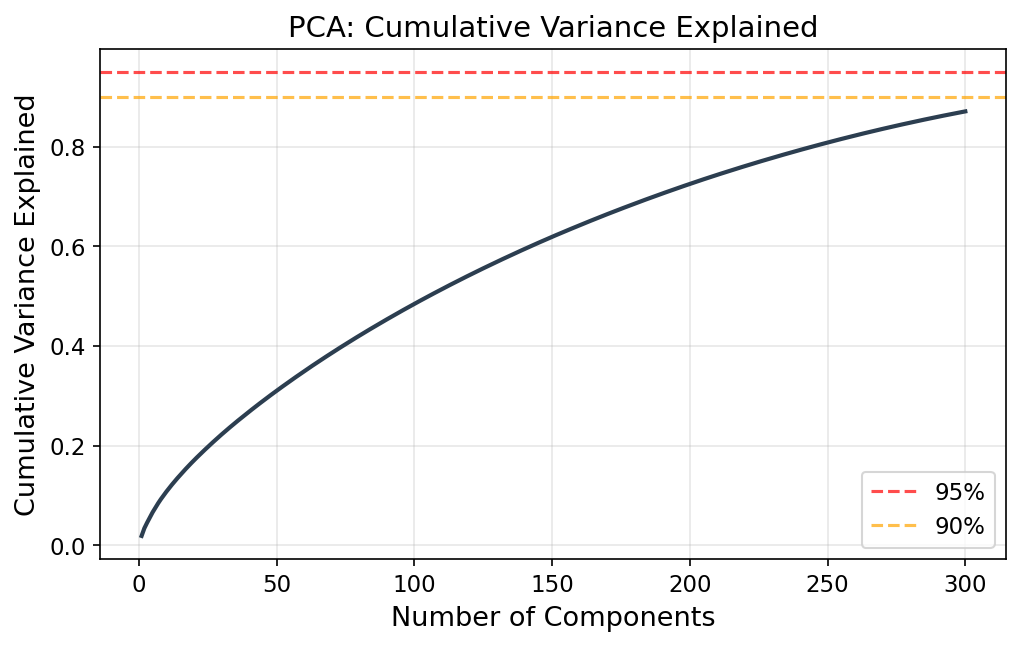
\includegraphics[width=\textwidth]{../figures/fig_pca_variance.png}
        \caption{Cumulative explained variance by PCA.}
        \label{fig:pca_var}
    \end{minipage}
    \hfill
    \begin{minipage}[t]{0.48\textwidth}
        \centering
        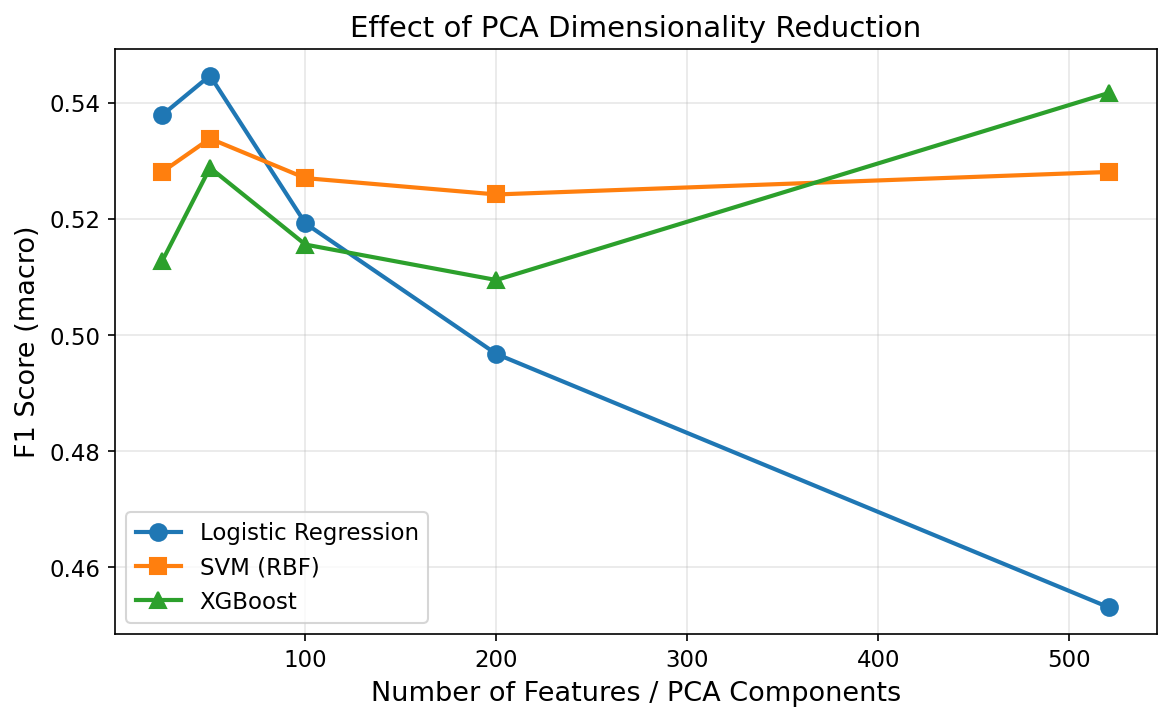
\includegraphics[width=\textwidth]{../figures/fig_pca_performance.png}
        \caption{Model performance vs.\ PCA components.}
        \label{fig:pca_perf}
    \end{minipage}
\end{figure}

The key finding is that \textbf{PCA-50 dramatically improves Logistic
Regression} from F1 = 0.453 to 0.545 (+20\%), making it competitive with
SVM and XGBoost. This reveals that LR's poor baseline performance stems
not from insufficient model capacity but from overfitting to
high-dimensional noise. PCA acts as a regularizer by projecting out
low-variance (likely noisy) directions.

SVM is relatively robust across dimensionalities, consistent with the
RBF kernel's implicit regularization through $\gamma = \text{scale}$.
XGBoost performs best with all 521 features because its tree-based
structure performs built-in feature selection by only splitting on
informative features.

% ── Experiment 5 ─────────────────────────────────────────────────────────────
\subsection{Experiment 5: Feature Ablation}

To quantify the contribution of each feature family, we compared
TF-IDF--only, handcrafted--only, and combined feature sets.

\begin{table}[H]
\centering
\caption{Feature ablation: macro-F1 by feature subset.}
\label{tab:ablation}
\small
\begin{tabular}{lccc}
\toprule
\textbf{Feature Set} & \textbf{LR} & \textbf{SVM} & \textbf{XGBoost} \\
\midrule
TF-IDF Only (500)        & 0.439          & 0.510          & 0.508          \\
Handcrafted Only (21)     & \textbf{0.518} & 0.511          & 0.513          \\
Combined (521)            & 0.453          & 0.528          & \textbf{0.542} \\
\bottomrule
\end{tabular}
\end{table}

\begin{figure}[H]
    \centering
    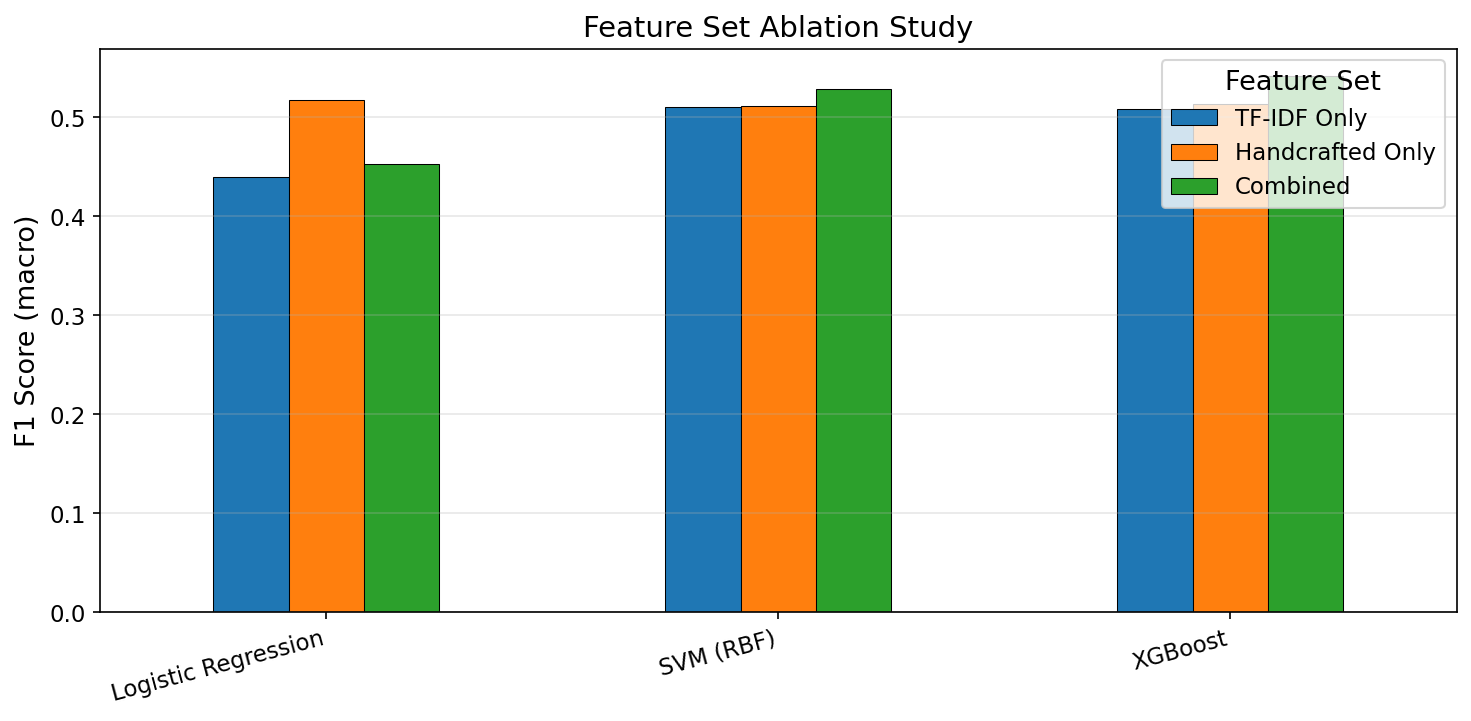
\includegraphics[width=0.55\textwidth]{../figures/fig_feature_ablation.png}
    \caption{Feature ablation comparison.}
    \label{fig:ablation}
\end{figure}

The most striking result is that \textbf{21 handcrafted features
outperform 500 TF-IDF features} for Logistic Regression (0.518 vs.\ 0.439)
and match SVM performance (0.511 vs.\ 0.510). This underscores the value
of domain-informed feature engineering: the handcrafted features distill
the linguistically relevant signal into a compact, low-noise
representation that linear models can exploit effectively.

For XGBoost, combining both feature families yields the best result
(0.542), suggesting that the ensemble learner benefits from both the
fine-grained lexical signal in TF-IDF and the high-level stylistic
signal in handcrafted features. The tree-based model can selectively
attend to informative features from either family while ignoring noise.

\begin{figure}[H]
    \centering
    \begin{minipage}[t]{0.48\textwidth}
        \centering
        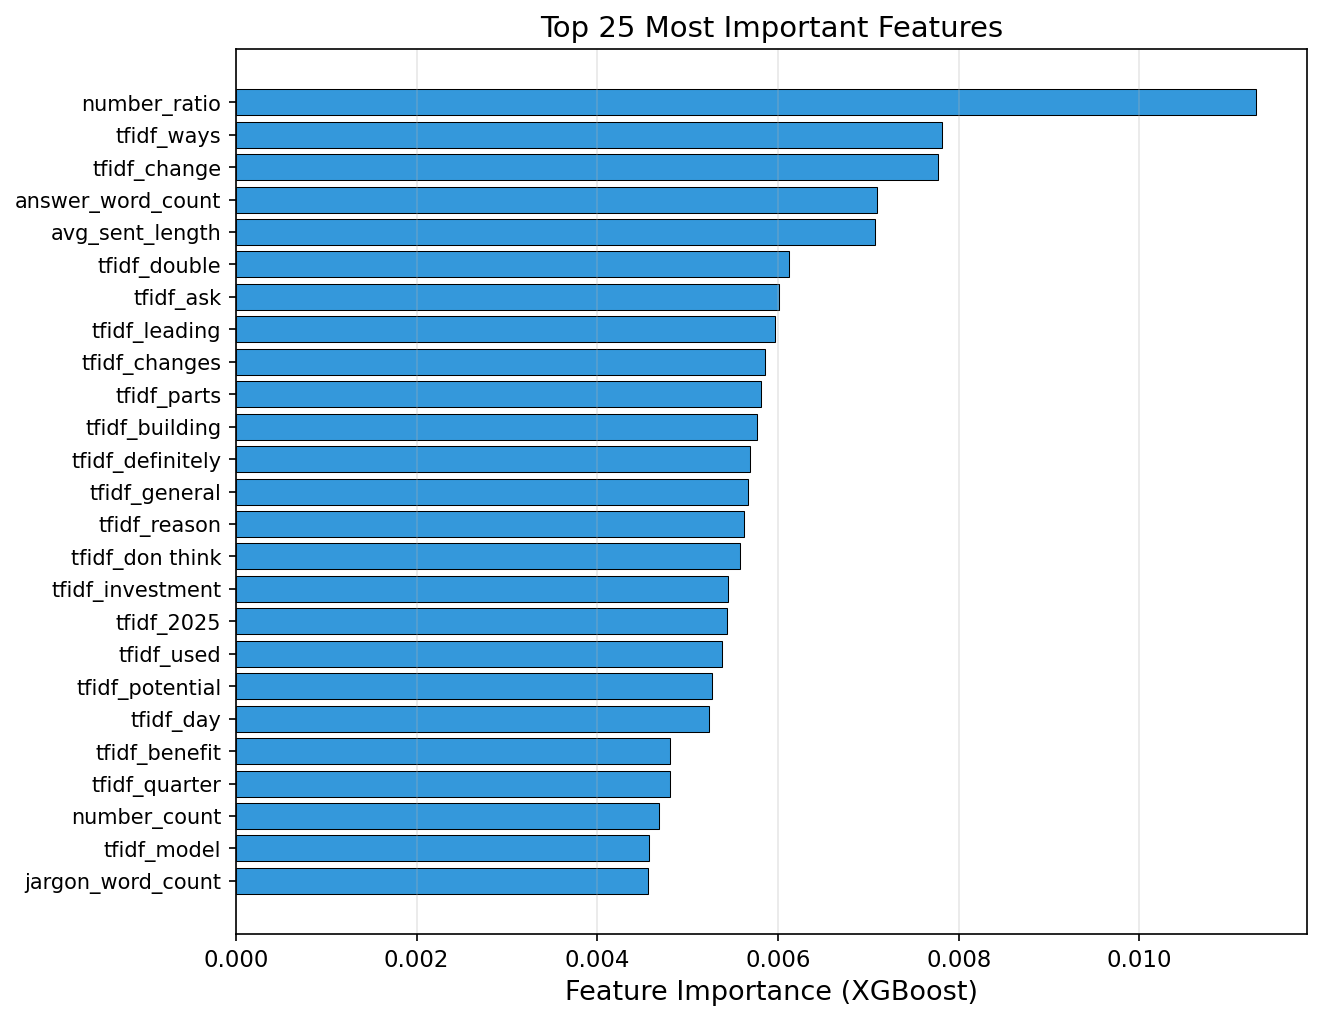
\includegraphics[width=\textwidth]{../figures/fig_feature_importance.png}
        \caption{Top features by XGBoost gain (full set).}
        \label{fig:feat_imp}
    \end{minipage}
    \hfill
    \begin{minipage}[t]{0.48\textwidth}
        \centering
        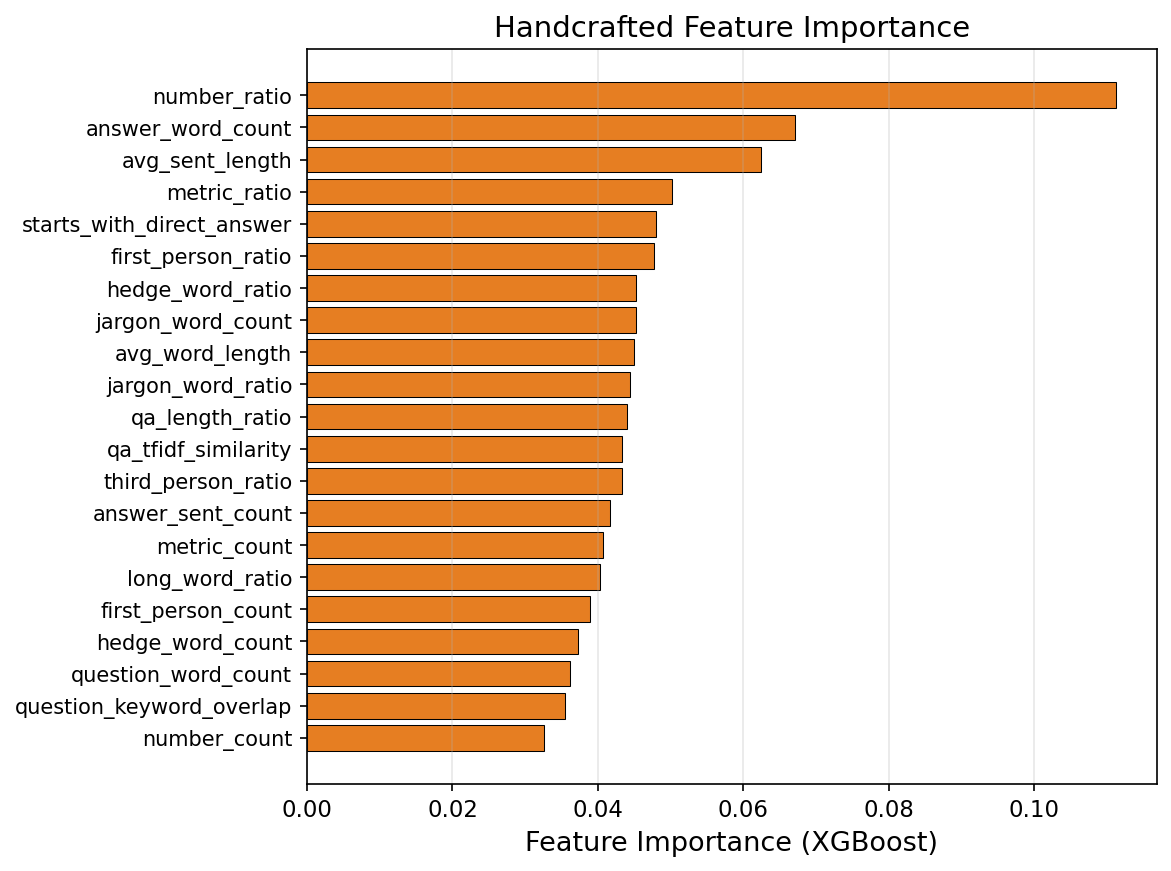
\includegraphics[width=\textwidth]{../figures/fig_handcrafted_importance.png}
        \caption{Handcrafted feature importance.}
        \label{fig:hc_imp}
    \end{minipage}
\end{figure}

Feature importance analysis (Figures~\ref{fig:feat_imp}
and~\ref{fig:hc_imp}) reveals that hedging and jargon ratios,
question--answer length ratio, and semantic similarity are among the
most discriminative handcrafted features---consistent with our
intuitions about what characterizes evasive communication.

% ── Experiment 6 ─────────────────────────────────────────────────────────────
\subsection{Experiment 6: LLM-Based Data Augmentation}
\label{sec:augment}

Motivated by the learning curve analysis showing that more data improves
performance, we explored LLM-based data augmentation using Qwen3-8B.
For each training sample, the model was prompted to rewrite answers with
a different communication style (e.g., \textsc{Evasive} $\to$
\textsc{Direct} and vice versa), generating new training samples with
known labels. This approach produces semantically meaningful augmentations
rather than surface-level perturbations.

\paragraph{Quality control.}
In practice, LLM rewriting can leak prompt text or chain-of-thought style
``thinking'' tokens into the output. We therefore post-processed generations to
remove \texttt{<think>...</think>} blocks (if present) and discarded samples
that appeared to echo instructions or chat-role scaffolding (e.g., \texttt{user},
\texttt{assistant}, or the rewrite prompt itself). This prevents the classifier
from learning artifacts unrelated to corporate communication style.

\paragraph{Status.}
Results from this augmentation experiment are pending completion and will be
inserted here (baseline vs.\ augmented performance, plus a brief analysis of
which classes benefit most).

% ─────────────────────────────────────────────────────────────────────────────
\section{Discussion}
\label{sec:discussion}
% ─────────────────────────────────────────────────────────────────────────────

\subsection{Expected vs.\ Observed Results}

We initially expected that fine-grained TF-IDF features would dominate
classification performance, with handcrafted features providing marginal
gains. The opposite proved true for linear models: 21 handcrafted features
outperformed 500 TF-IDF features for Logistic Regression and matched SVM.
This finding highlights a core lesson in machine learning: \emph{fewer,
higher-quality features often outperform many noisy features}, especially
when data is limited.

DistilBERT's lead over all classical models (F1 = 0.570 vs.\ 0.542)
was expected but modest. Pre-trained language models have access to
contextual and semantic information that bag-of-words representations
discard, yet the advantage is limited by the small dataset and noisy
labels.

\subsection{Factors Affecting Performance}

\paragraph{Label noise.} The primary performance bottleneck is label
quality. LLM-generated labels via zero-shot prompting inevitably
contain systematic errors, particularly for ambiguous cases where
evasiveness and jargon overlap. Human annotation would likely improve
absolute performance but was infeasible at scale for this project.

\paragraph{Class overlap.} The confusion matrices reveal substantial
overlap between \textsc{Evasive} and \textsc{Jargon} classes. This is
linguistically motivated: both categories involve non-specific,
non-committal language, differing primarily in whether the vagueness
is achieved through hedging or through technical terminology. A
two-class formulation (Direct vs.\ Non-Direct) might yield higher
accuracy but would sacrifice granularity.

\paragraph{Dataset size.} At $n = 1{,}129$, the dataset is in the
regime where overfitting is a significant concern, particularly for
high-dimensional TF-IDF representations. The PCA experiment confirms
this: aggressive dimensionality reduction substantially improves
linear model performance.

\subsection{Key Takeaways}

\begin{enumerate}[nosep]
    \item \textbf{Feature engineering matters.} Domain-specific handcrafted
          features provided more discriminative power per dimension than
          TF-IDF for linear models, demonstrating the value of injecting
          domain knowledge into the feature pipeline.
    \item \textbf{Dimensionality reduction as regularization.} PCA-50
          improved LR by 20\%, revealing that the model's poor baseline was
          due to overfitting, not underfitting. This is a practical lesson
          for practitioners working with limited data.
    \item \textbf{Class balance is not always the issue.} SMOTE had
          negligible impact because the dataset was already balanced---a
          reminder to diagnose the actual bottleneck before applying
          standard remedies.
    \item \textbf{Pre-trained models help but are not magic.} DistilBERT
          outperformed classical models by $\sim$4 F1 points, but noisy
          labels limit all methods equally.
\end{enumerate}

\subsection{Future Work}

Several directions could improve performance: (1)~obtaining human
annotations for a subset of the data to calibrate the LLM labeler and
quantify label noise; (2)~using larger pre-trained models (e.g., full
BERT or domain-specific FinBERT) with more extensive hyperparameter
tuning; (3)~expanding the dataset with more companies and time periods;
and (4)~exploring semi-supervised or active learning approaches that
leverage the large volume of unlabeled transcript text.

\subsection{Remaining Questions}
While the experiments answer our core question (the task is learnable and
DistilBERT helps under noisy labels), several open questions remain:
(1)~\textbf{What fraction of labels are wrong, and where?} Without a
human-annotated subset, we cannot quantify the LLM annotator's error modes
or estimate the attainable upper bound.
(2)~\textbf{Is ``Evasive'' vs.\ ``Jargon'' a reliable distinction?} The confusion
matrices suggest substantial class overlap; it is unclear whether the boundary
is linguistically sharp or an artifact of our labeling rubric.
(3)~\textbf{How much of the signal is semantic vs.\ stylistic?} Our handcrafted
features target style (hedging, numbers, jargon), but a model might also pick up
topic cues (e.g., guidance, tariffs). Disentangling these would require controls
or counterfactual evaluation.
(4)~\textbf{Does performance generalize across time, sectors, and companies?}
Cross-validation mixes companies and quarters; a stricter split (e.g., hold out
companies or years) may reduce scores and better reflect real deployment.

% ─────────────────────────────────────────────────────────────────────────────
\section*{References}
\addcontentsline{toc}{section}{References}
% ─────────────────────────────────────────────────────────────────────────────

\begin{thebibliography}{10}

\bibitem{sklearn}
F.~Pedregosa et al.,
``Scikit-learn: Machine learning in Python,''
\emph{Journal of Machine Learning Research}, vol.~12, pp.~2825--2830, 2011.

\bibitem{xgboost}
T.~Chen and C.~Guestrin,
``XGBoost: A scalable tree boosting system,''
in \emph{Proc.\ 22nd ACM SIGKDD}, pp.~785--794, 2016.

\bibitem{distilbert}
V.~Sanh, L.~Debut, J.~Chaumond, and T.~Wolf,
``DistilBERT, a distilled version of BERT: smaller, faster, cheaper and lighter,''
\emph{arXiv preprint arXiv:1910.01108}, 2019.

\bibitem{smote}
N.~V.~Chawla, K.~W.~Bowyer, L.~O.~Hall, and W.~P.~Kegelmeyer,
``SMOTE: Synthetic Minority Over-sampling Technique,''
\emph{Journal of Artificial Intelligence Research}, vol.~16, pp.~321--357, 2002.

\bibitem{seekingalpha}
SeekingAlpha,
``Earnings call transcripts,''
\url{https://seekingalpha.com}, accessed 2025.

\bibitem{qwen}
Qwen Team,
``Qwen technical report,''
\emph{arXiv preprint arXiv:2309.16609}, 2023.

\bibitem{tfidf}
G.~Salton and C.~Buckley,
``Term-weighting approaches in automatic text retrieval,''
\emph{Information Processing \& Management}, vol.~24, no.~5, pp.~513--523, 1988.

\bibitem{transformers}
T.~Wolf et al.,
``Transformers: State-of-the-art natural language processing,''
in \emph{Proc.\ EMNLP 2020: System Demonstrations}, pp.~38--45, 2020.

\end{thebibliography}

% ─────────────────────────────────────────────────────────────────────────────
% APPENDIX — Code Listing (does not count toward page limit)
% ─────────────────────────────────────────────────────────────────────────────
\clearpage
\appendix
\section*{Appendix: Core Code Excerpts (Annotated)}
\addcontentsline{toc}{section}{Appendix: Code Listing}

\noindent The repository contains full, runnable scripts. For readability, we
excerpt the most important logic from each stage below (with brief
intent-oriented comments).

\subsection*{Configuration (\texttt{config.py})}
\begin{lstlisting}[caption={Core configuration knobs (API limits, CV, features).}]
# Centralized configuration for reproducibility
RAPIDAPI_HOST = "seeking-alpha.p.rapidapi.com"
MAX_API_CALLS = 480
TRANSCRIPTS_PER_TICKER = 8

TFIDF_MAX_FEATURES = 500
CV_FOLDS = 5
RANDOM_STATE = 42
\end{lstlisting}

\subsection*{Crawling (\texttt{01\_crawl\_transcripts.py})}
\begin{lstlisting}[caption={Robust API GET with retry + saving transcript HTML.}]
def api_get(path: str, params: dict) -> dict:
    # Retry + exponential backoff for transient RapidAPI failures
    for attempt in range(MAX_RETRIES):
        try:
            conn.request("GET", f"{path}?{urlencode(params)}", headers=headers)
            resp = conn.getresponse()
            if resp.status == 200:
                return json.loads(resp.read().decode("utf-8"))
        except Exception:
            pass
        time.sleep(BASE_SLEEP * (2 ** attempt))
    raise RuntimeError(f"API failed: {path}")

# (1) list transcript IDs per ticker, (2) fetch details, (3) store raw HTML/json
\end{lstlisting}

\subsection*{Q\&A Extraction (\texttt{02\_extract\_qa\_pairs.py})}
\begin{lstlisting}[caption={Locate Q\&A section and pair analyst question -> executive answer.}]
qa_pairs = []
for turn in speaker_turns:
    # Analysts ask; executives answer next
    if is_analyst(turn.speaker) and looks_like_question(turn.text):
        q = turn.text
        a = next_executive_answer(turn)
        if a:
            qa_pairs.append({"question": q, "answer": a, "ticker": ticker})
\end{lstlisting}

\subsection*{LLM Labeling (\texttt{03\_llm\_annotate.py})}
\begin{lstlisting}[caption={Prevent ``thinking'' leakage and parse a 3-class label.}]
def strip_thinking(text: str) -> str:
    # Qwen can emit <think>...</think>; remove it for robust label parsing
    text = re.sub(r"<think>.*?</think>", "", text, flags=re.DOTALL)
    text = re.sub(r"<\|.*?\|>", "", text)  # strip special tokens
    return text.strip()

prompt = tokenizer.apply_chat_template(messages, tokenize=False,
                                       add_generation_prompt=True,
                                       enable_thinking=False)
raw = model.generate(...)
label = parse_label(strip_thinking(decoded_text))
\end{lstlisting}

\subsection*{Feature Building (\texttt{04\_build\_dataset.py})}
\begin{lstlisting}[caption={Two families: TF-IDF (500) + handcrafted (21).}]
# TF-IDF: lexical cues from concatenated question+answer
X_tfidf = TfidfVectorizer(max_features=500, ngram_range=(1, 2)).fit_transform(text)

# Handcrafted: style/specificity cues (hedging, jargon ratio, numbers, similarity)
X_hc = np.column_stack([hedge_ratio, jargon_ratio, number_ratio, qa_tfidf_sim, ...])

X = hstack([X_tfidf, X_hc])  # final feature matrix
\end{lstlisting}

\subsection*{Experiments (\texttt{05\_experiments.py})}
\begin{lstlisting}[caption={Stratified 5-fold CV + metrics + one-vs-rest AUROC.}]
skf = StratifiedKFold(n_splits=5, shuffle=True, random_state=42)
scores = cross_validate(model_pipeline, X, y, cv=skf,
                        scoring={"acc": "accuracy", "f1": f1_macro})

# AUROC (one-vs-rest): compute per class, then macro-average
for c in range(3):
    fpr, tpr, _ = roc_curve(y_bin[:, c], y_score[:, c])
    auc_c = auc(fpr, tpr)
\end{lstlisting}

\subsection*{Augmentation (\texttt{06\_augment\_data.py})}
\begin{lstlisting}[caption={Style rewriting + artifact filtering for clean synthetic data.}]
# Rewrite EVASIVE -> DIRECT and DIRECT -> EVASIVE using Qwen prompts.
# Post-process to remove <think> blocks and reject prompt/role echoes.
new_text = strip_thinking(generated)
if is_valid_rewrite(new_text):
    augmented_rows.append({...})
\end{lstlisting}

\end{document}
